\question[15] A 0.6 kg block of ice is sliding by you on a very slippery floor at 3.5 m/s. As it goes by, you give it a kick perpendicular to its path. Your foot is in contact with the ice block for 0.002 seconds. The block eventually slides at an angle of $\theta=24^\circ$ from its original direction. What force did you apply during the kick? Make sure to express your result as a vector.

\begin{figure}[ht!]
	\centering
	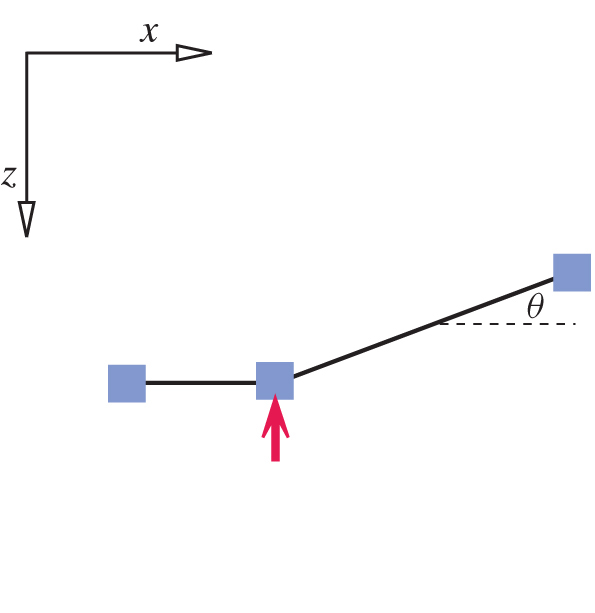
\includegraphics[width=8cm]{iceblock.jpg}
\end{figure}